\chapter{Podręcznik użytkownika}
\label{cha:podrecznik uzytkownika}

Poniżej opisane są kroki umożliwiające szybkie i bezproblemowe uruchomienie stworzonej aplikacji w środowisku lokalnym. 

%------------------------------------------------------------------------------------------------

\section{Wymagania dotyczące środowiska pracy}
Aby korzystać z zaimplementowanej aplikacji niezbędne jest:
\begin{itemize}
\item środowisko z systemem operacyjnym OSX lub Linux
\item środowisko z zainstalowanym interpreterem języka Ruby w wersji 2.1.5
\item dostęp do internetu w celu pobrania zależności projektu.
\item przeglądarka internetowa z włączoną obsługą języka JavaScript.
\end{itemize}
Jeżeli środowisko jest wyposażone w powyższe elementy, należy pobrać wszystkie zależności za pomocą polecenia \textit{bundle install}, oraz uruchomić serwer poleceniem \textit{bundle exec rail s}. Aplikacja zostanie uruchomiona na serwerze lokalnym w domyślnej konfiguracji. Aby otworzyć aplikację w przeglądarce, należy wpisać adres \textit{localhost:3000}.

%------------------------------------------------------------------------------------------------

\newpage

\section{Rejestracja}
\label{sec:rejestracja}
Aby się zarejestrować, należy kliknąć lewym przyciskiem myszy na przycisku \quotes{Registration} znajdującym się w prawym górnym rogu aplikacji. Po kliknięciu na ekranie powinno pojawić się dodatkowe okno z formularzem rejestracji. Po poprawnym wypełnieniu formularza rejstracji, użytkownik powinien od razu zostać zalogowany do systemu.\\
\\
\begin{minipage}{\linewidth}
\makebox[\linewidth]{
  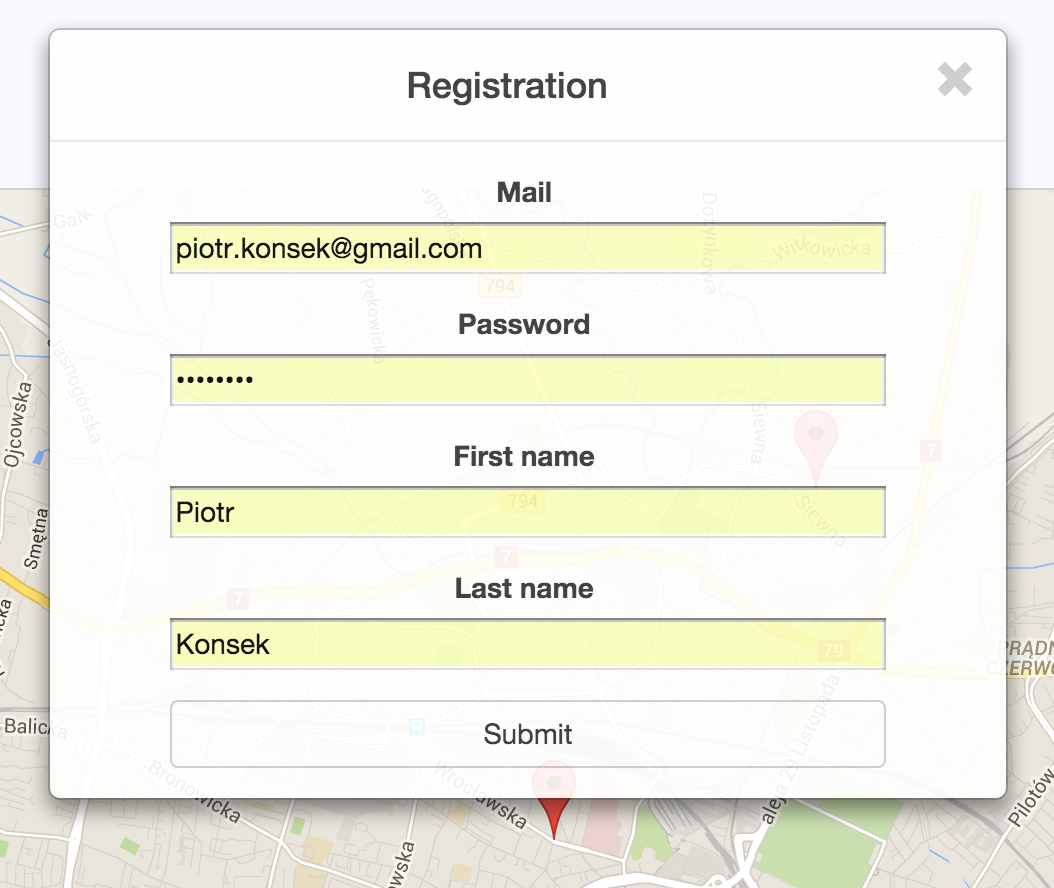
\includegraphics[keepaspectratio=true,scale=0.8]{pictures/registration.png}}
\captionof{figure}{Rejestracja}\label{registration}
\end{minipage}\\

\newpage

%------------------------------------------------------------------------------------------------

\section{Logowanie}
\label{sec:logowanie}
Aby się zalogować, należy kliknąć lewym przyciskiem myszy na przycisku \quotes{Login} znajdującym się również w prawym górnym rogu formularza obok przycisku służącego do rejestracji. Po jego naciśnięciu, na ekranie powinno pojawić się dodatkowe okienko z formularzem logowania. Po poprawnym wypełnieniu formularza oraz autentykacji, użytkownik powinien zostać zalogowany do sytstemu. 
Po zalogowaniu użytkownika na pasku powinny pojawić się przycisku służące do dodania nowej oferty, edycji profilu użytkownika oraz wylogowania się.\\
\\

\begin{minipage}{\linewidth}
\makebox[\linewidth]{
  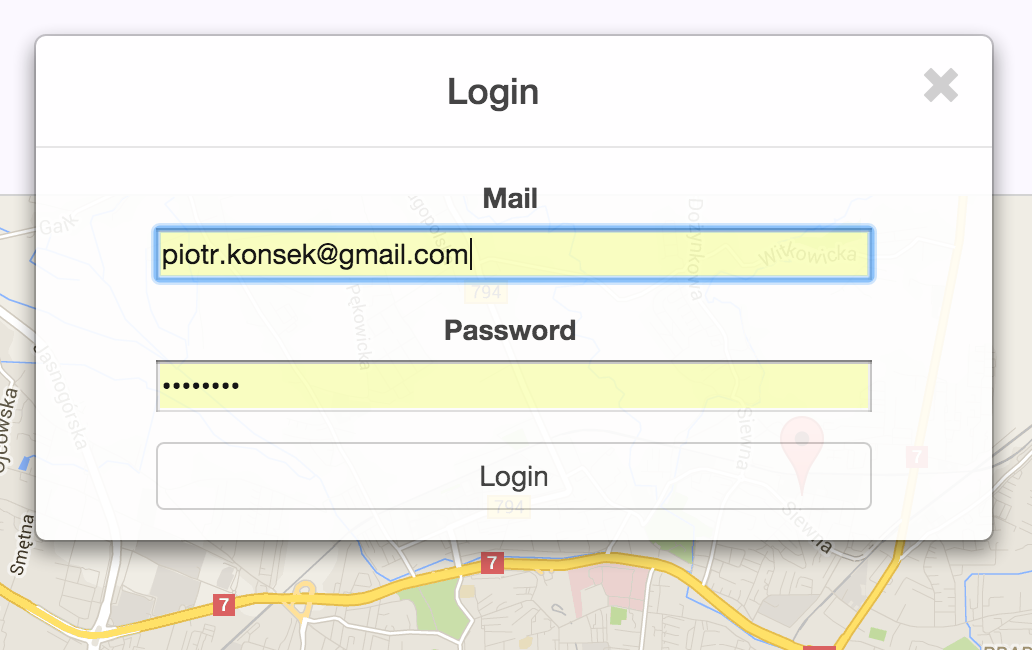
\includegraphics[keepaspectratio=true,scale=0.8]{pictures/login.png}}
\captionof{figure}{Logowanie}\label{login}
\end{minipage}\\

\newpage

%------------------------------------------------------------------------------------------------

\section{Dodanie oferty}
Aby dodać nową ofertę, należy kliknąć lewym przyciskiem myszy na przycisk opatrzony nazwą \quotes{Add offer}. Po kliknięciu powinien pojawić się okno z formularzem umożliwiającym wpisania danych.\\
\\
\begin{minipage}{\linewidth}
\makebox[\linewidth]{
  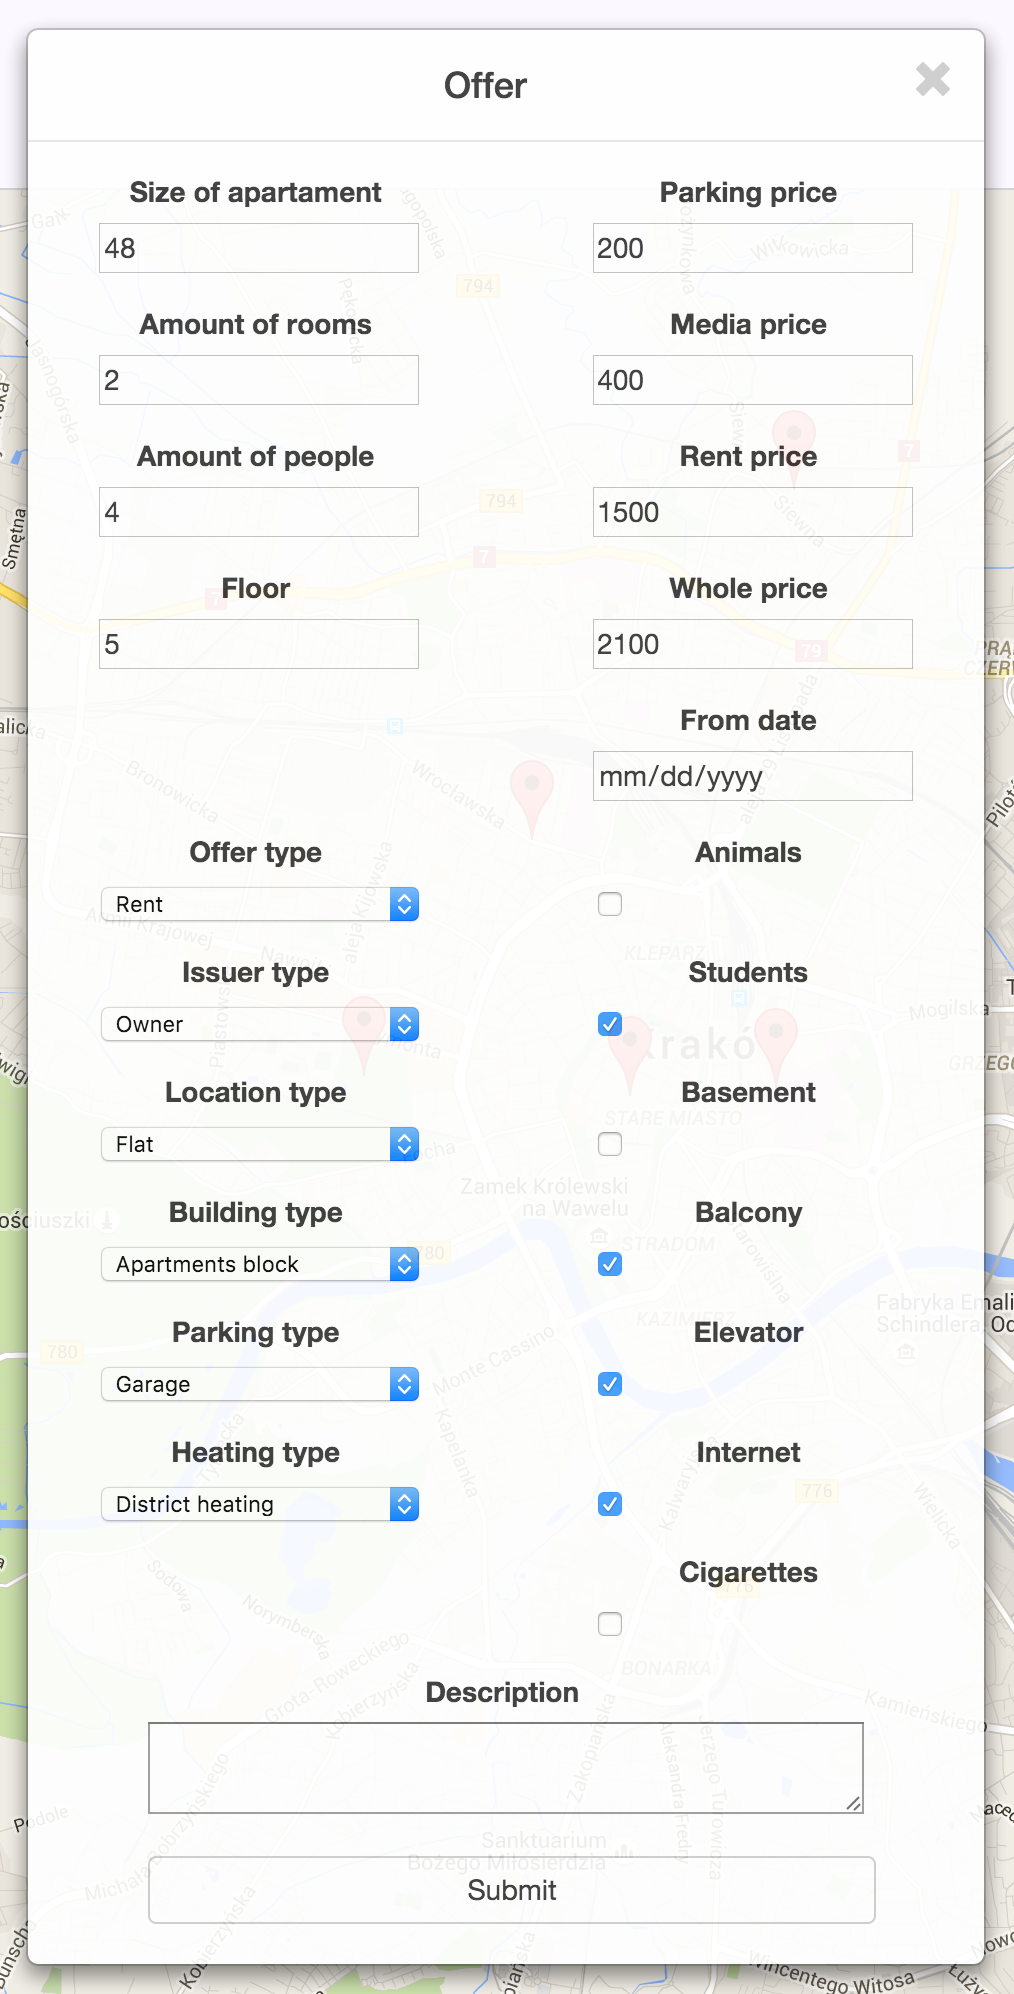
\includegraphics[keepaspectratio=true,scale=0.5]{pictures/add-offer1.png}}
\captionof{figure}{Dodawanie nowej oferty}\label{add-offer1}
\end{minipage}\\

\newpage

Po kliknięciu przycisku \quotes{Submit} i poprawnej walidacji, użytkownik zostaje przeniesiony do okna umożliwiającego dodawanie zdjęć. Po wybraniu zdjęcia należy kliknąć przycisk \quotes{Create Photo} aby wysłać zdjęcie na serwer. Po poprawnej operacji zapisu zdjęcia, powinno się ono pojawić na górze formularza. Mały przycisk w kształcie litery X przy zdjęciu służy do jego usuwania.\\
\\
\begin{minipage}{\linewidth}
\makebox[\linewidth]{
  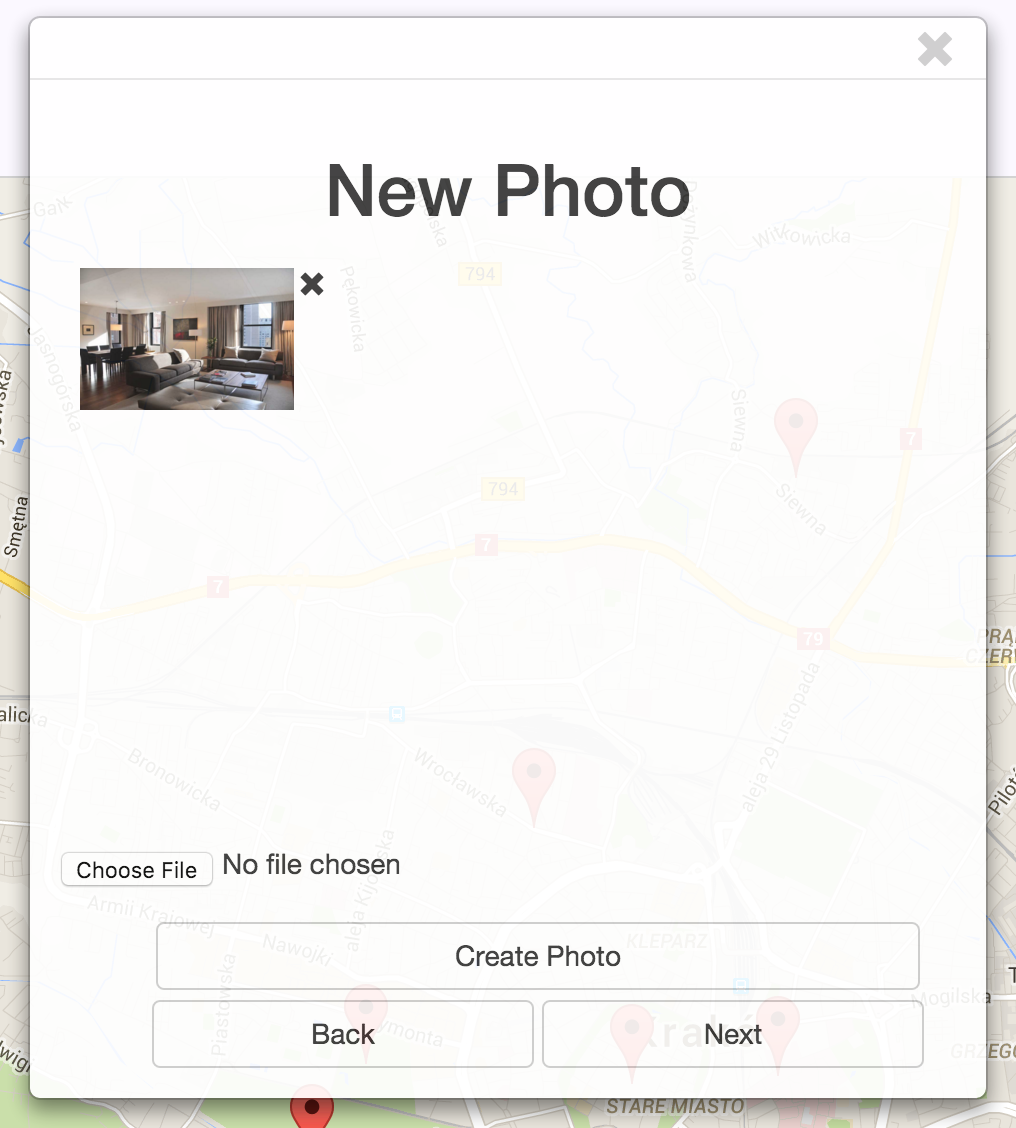
\includegraphics[keepaspectratio=true,scale=0.6]{pictures/add-offer2.png}}
\captionof{figure}{Dodawanie zdjęć do oferty}\label{add-offer2}
\end{minipage}\\

\newpage

Po kliknięciu przycisku \quotes{Next} użytkownik zostaje przeniesiony do ostatniego etapu tworzenia nowego ogłoszenia, w którym musi określić precyzjną lokalizację oferty. Dokładną lokalizację użytkownik może wybrać poprzez kliknięcie na mapie. W ten sposób zostaje określona długość i szerokość geograficzna. Po wypełnieniu pozostałych pól formularza i kliknięciu przycisku \quotes{Submit}, oferta powinna pojawić się na głównej mapie.\\
\\
\begin{minipage}{\linewidth}
\makebox[\linewidth]{
  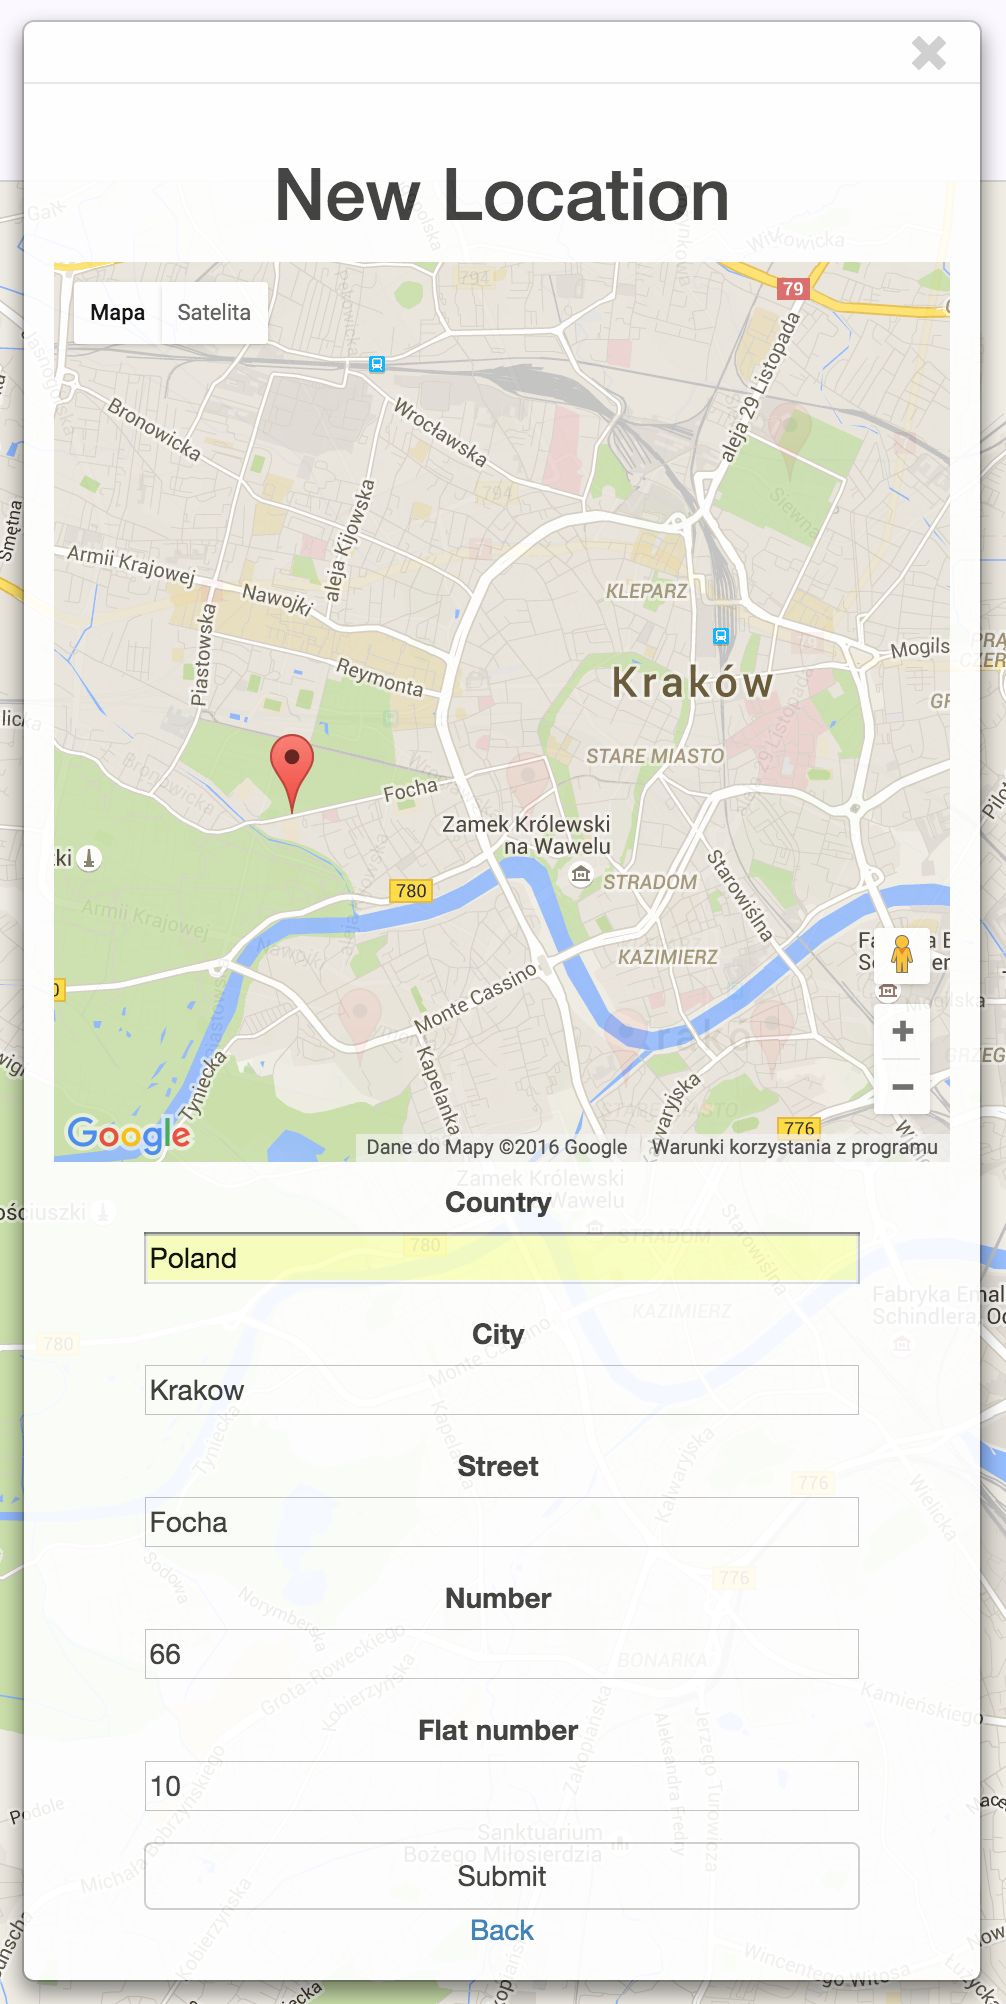
\includegraphics[keepaspectratio=true,scale=0.5]{pictures/add-offer3.png}}
\captionof{figure}{Określanie lokalizacji oferty}\label{add-offer3}
\end{minipage}\\

%------------------------------------------------------------------------------------------------

\section{Edycja oferty}
Jeżeli użytkownik naciśnie lewym klawiszem myszki na marker znajdujący się na głównej mapie, powinno się otworzyć okienko przedstawiające informacje o ofercie. Jeżeli dana oferta należy do użytkownika to oprócz informacji widocznych dla innych użytkowników, dostępny jest dla niego przycisk \quotes{Edit offer}, który przenosi użytkownika do formularza edycji oferty. \ref{delete-offer}\\
\\
\begin{minipage}{\linewidth}
\makebox[\linewidth]{
  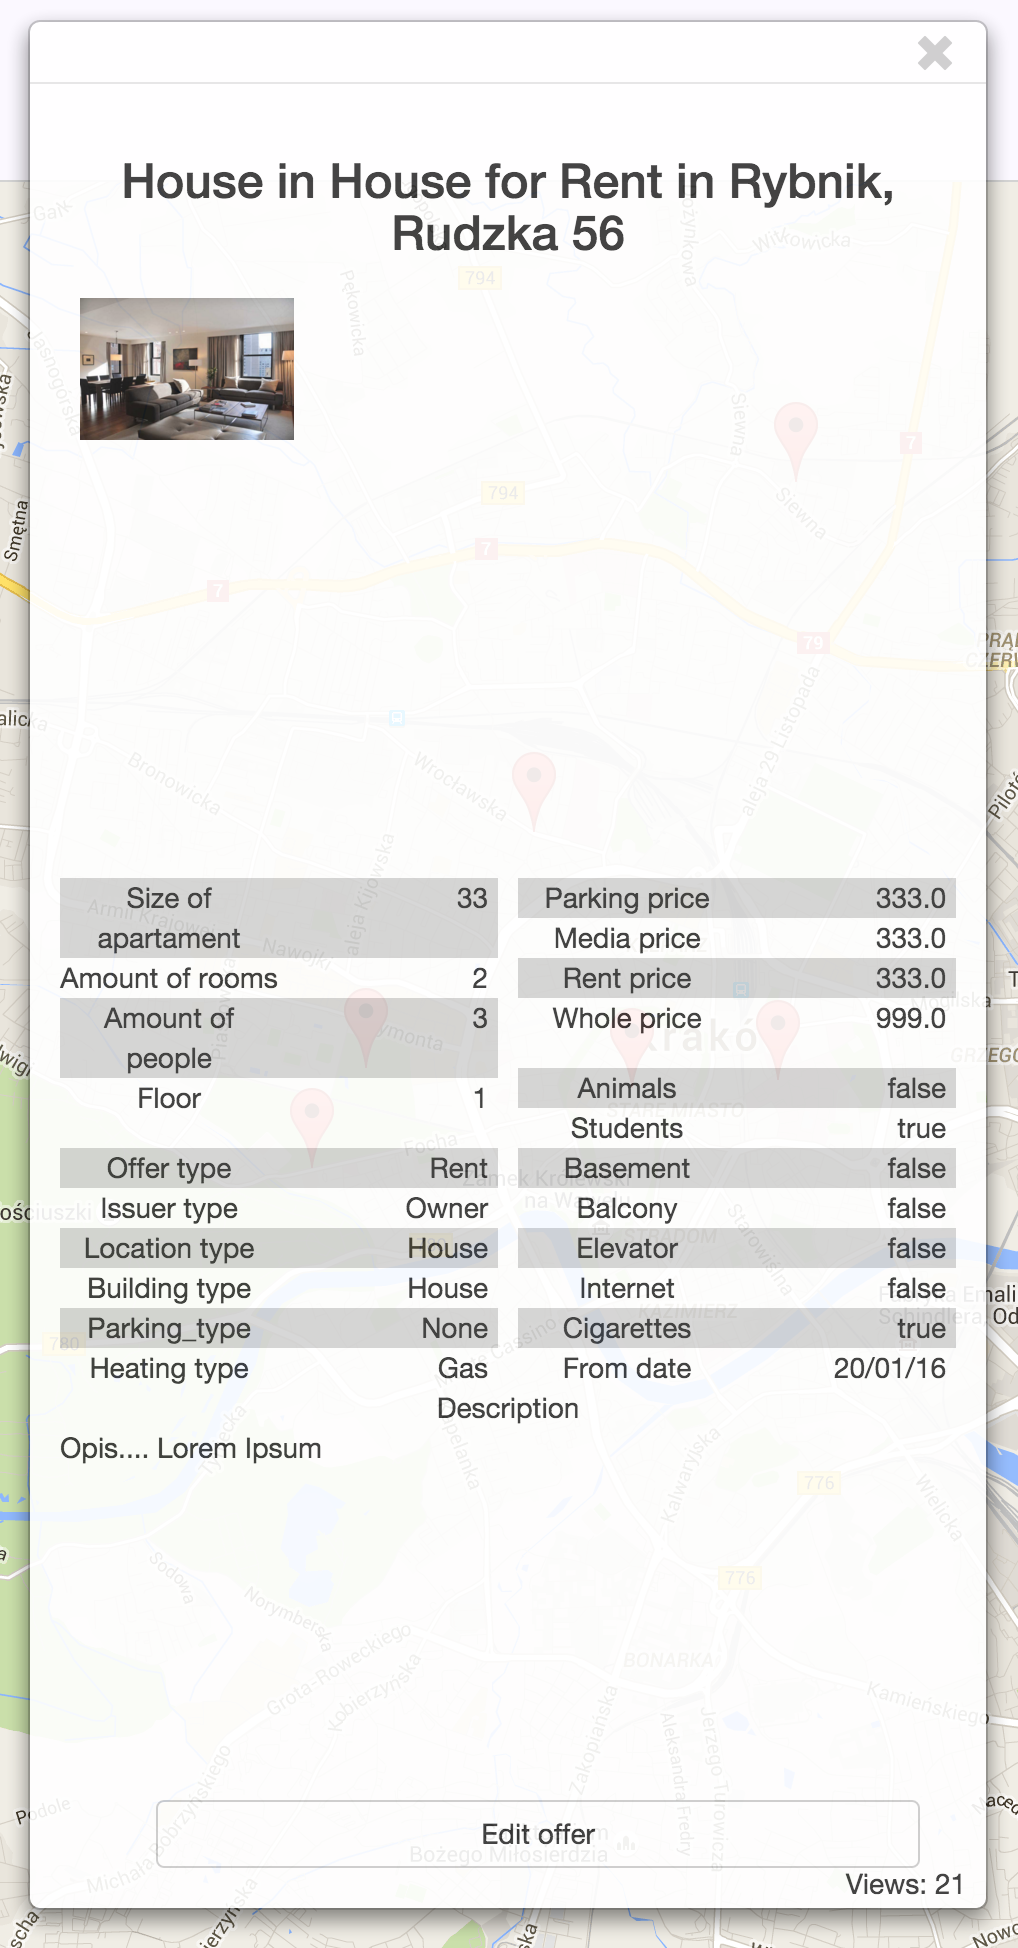
\includegraphics[keepaspectratio=true,scale=0.5]{pictures/edit-offer.png}}
\captionof{figure}{Edytowanie oferty}\label{edit-offer}
\end{minipage}\\

%------------------------------------------------------------------------------------------------

\section{Usunięcie oferty}
Po otworzeniu okna edycji oferty, na dole strony widoczny jest przycisk służący do usuwania danej oferty. Usunięcie oferty wiąże się z usunięciem wszystkich zdjęć i lokalizacji dołączonych do oferty.\\
\\
\begin{minipage}{\linewidth}
\makebox[\linewidth]{
  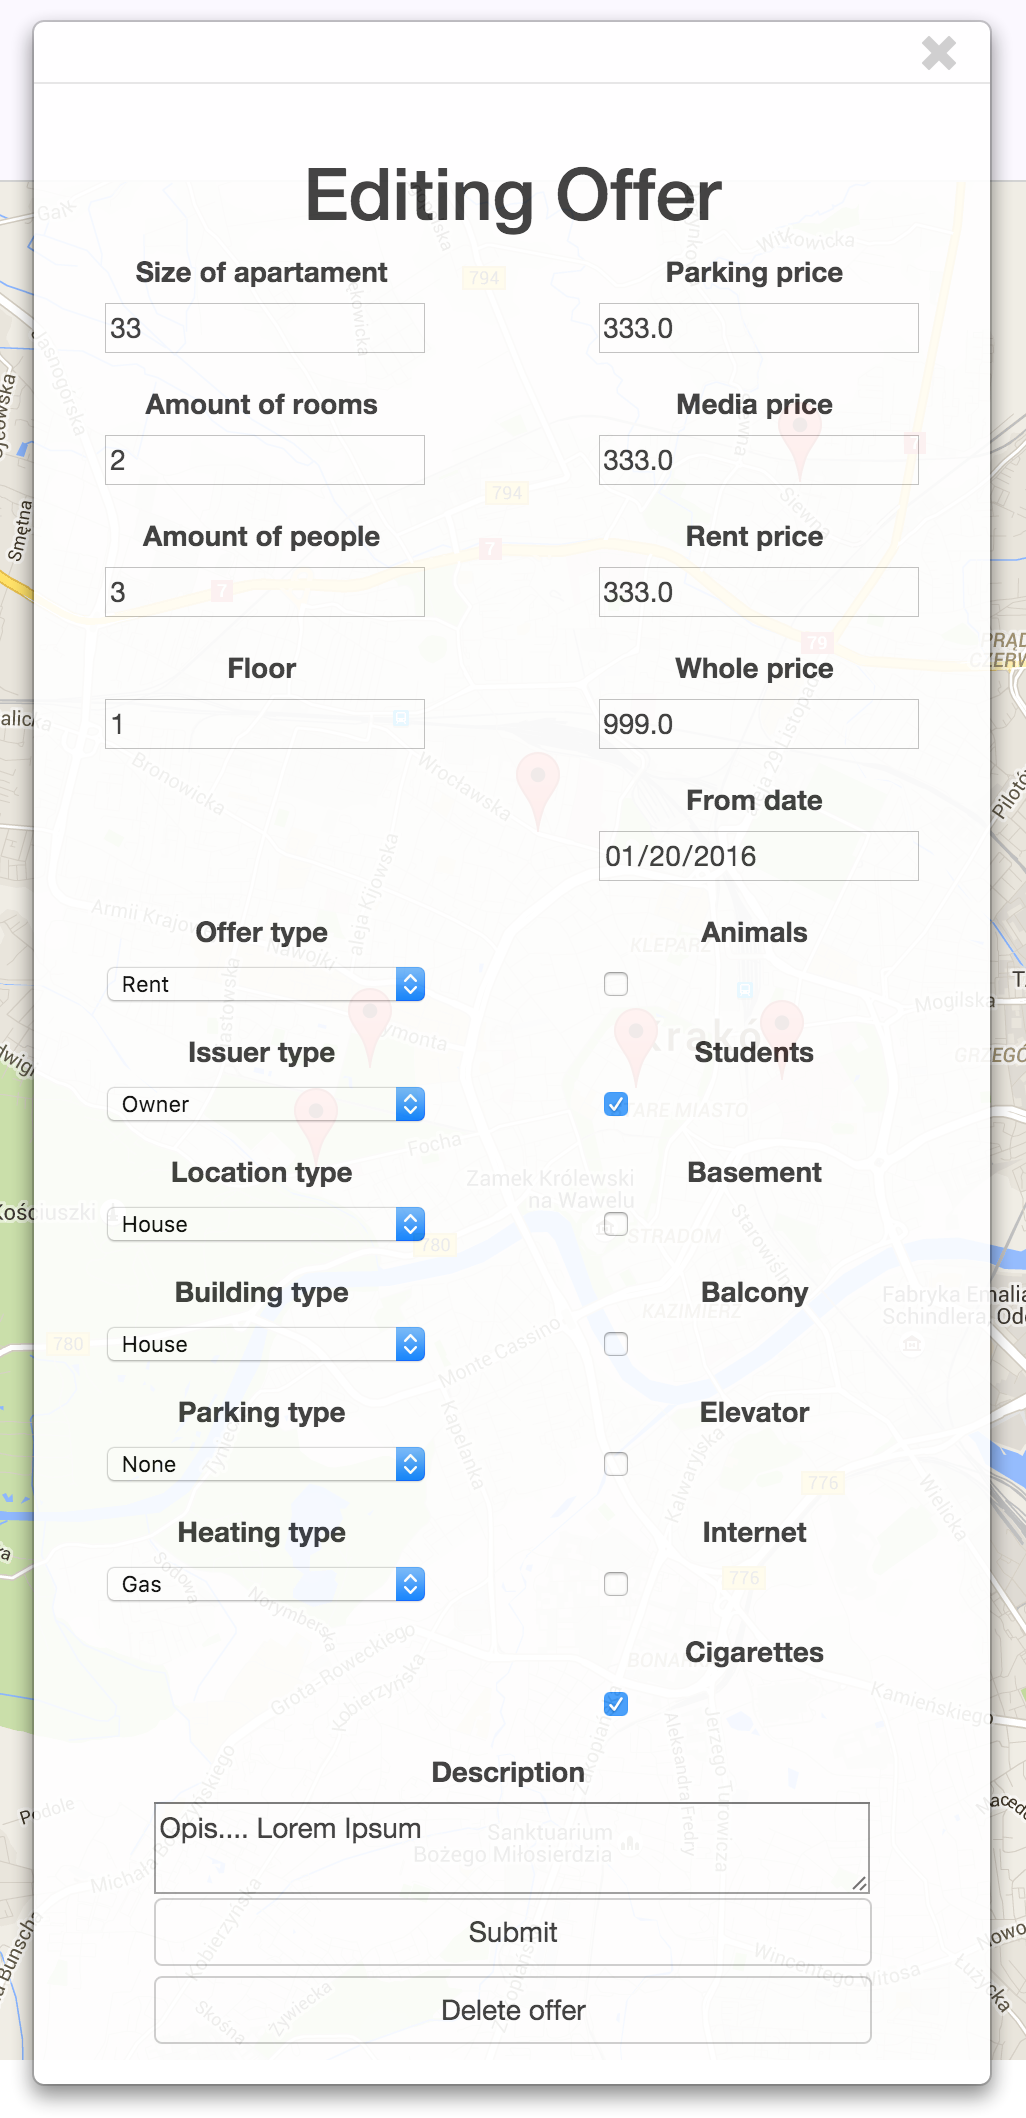
\includegraphics[keepaspectratio=true,scale=0.5]{pictures/delete-offer.png}}
\captionof{figure}{Usuwanie oferty}\label{delete-offer}
\end{minipage}\\ 

%------------ FILTROWANIE WYNIKÓW ----------------

\section{Filtrowanie wyników}
Filtrowanie wyników jest opcją dostępną zarówno dla niezalogowanych jak i zalogowanych użytkowników. Filtry znajdują się po lewej stronie aplikacji na liście z możliwością chowania. Jedyną różnicą pomiędzy używaniem filtrów dla użytkowników, to możliwość zapisania filtrów przez zalogowanego użytkownika. Po kliknięciu myszką na mapę, pojawia się na niej znacznik w kształcie okręgu. Jest to znacznik środka obszaru zainteresowań użytkownika. Promień tego obszaru użytkownik może zmieniac za pomocą pierwszego suwaka na liście filtrów. Pozostałe filtry odnoszą się bezpośrednio do atrybutów oferty.\\
\\
\begin{minipage}{\linewidth}
\makebox[\linewidth]{
  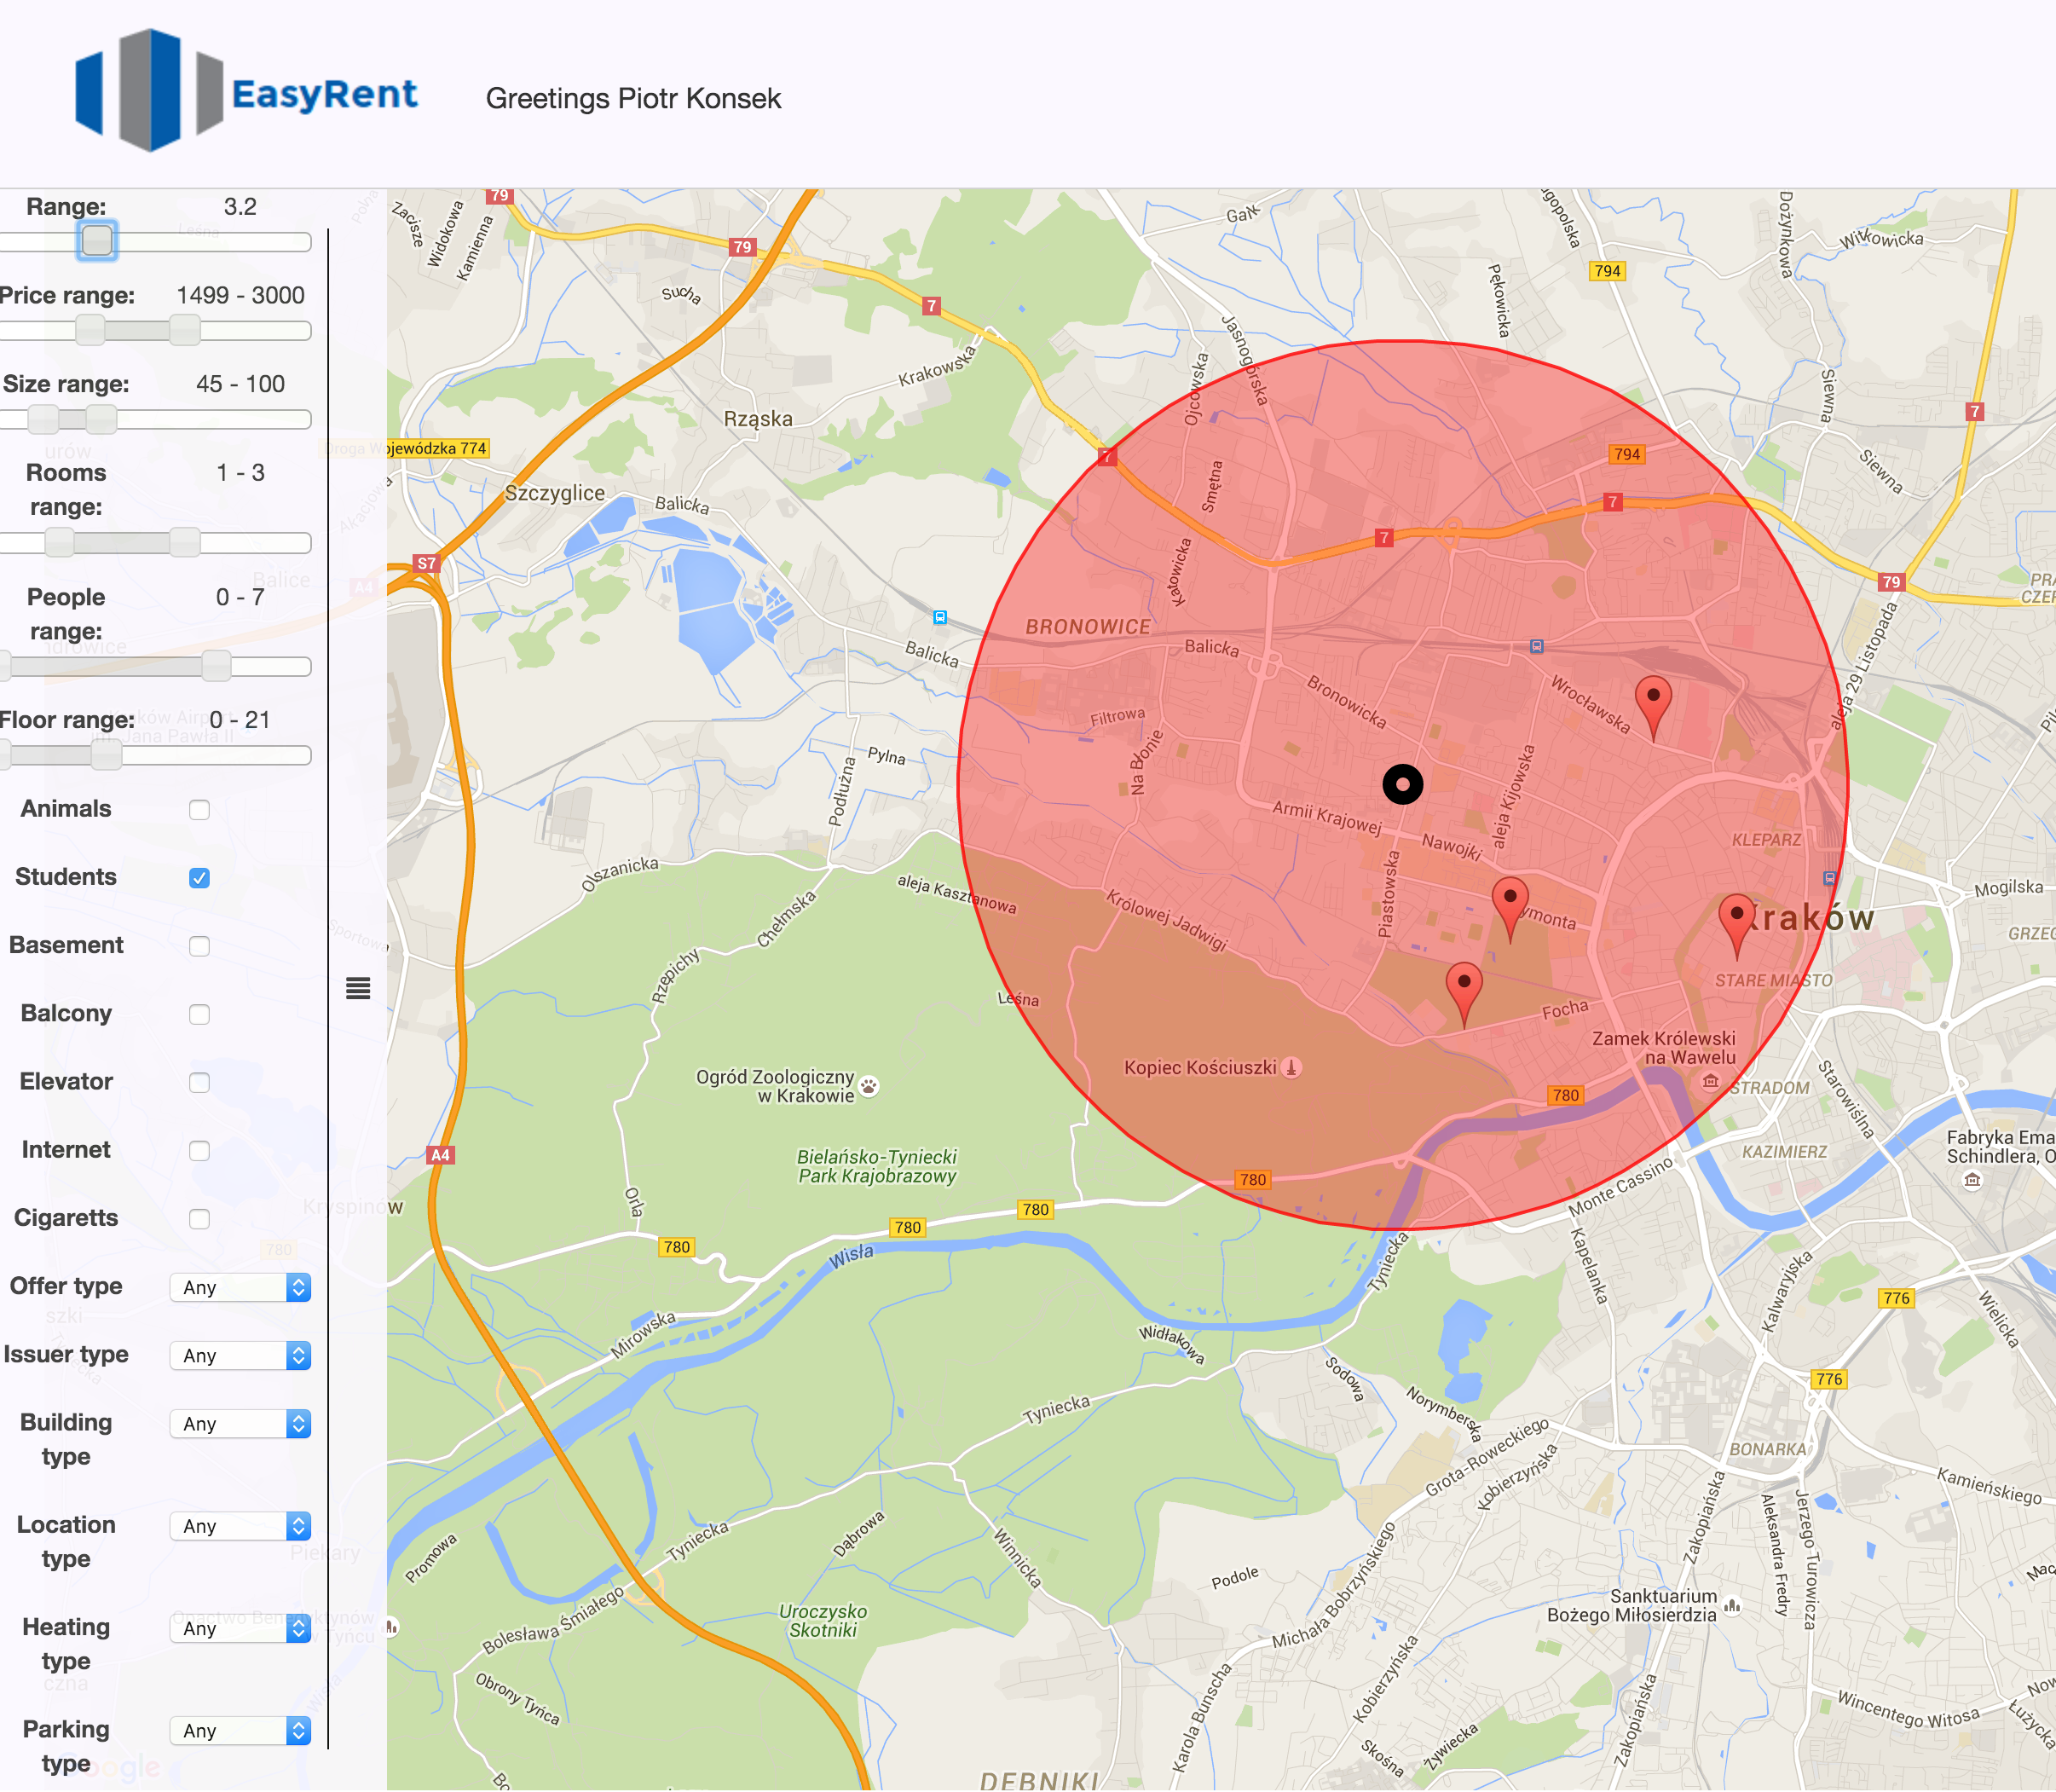
\includegraphics[keepaspectratio=true,scale=0.4]{pictures/filters.png}}
\captionof{figure}{Filtrowanie ofert}\label{filters}
\end{minipage}\\ 

%------------  WATCHED OFFERS ----------------

\section{Dodanie oferty do obserwowanych}
Jeżeli użytkownik naciśnie lewym klawiszem myszki na marker znajdujący się na głównej mapie, powinno się pojawiić okienko przedstawiające ofertę. Jeżeli dana oferta nie należy do użytkownika wtedy nie zostanie wyświetlony przycisk służący do przejścia do edycji oferty. Pojawi się natomiast przycisk służący do dodania oferty do obserwowanych ofert. Po kliknięciu tego przycisku i dodaniu oferty do obserwowanych, zmieni się on w przycisk służący odwrotnej akcji, czyli usunięcia oferty z listy obserwowanych.\\
\\
\begin{minipage}{\linewidth}
\makebox[\linewidth]{
  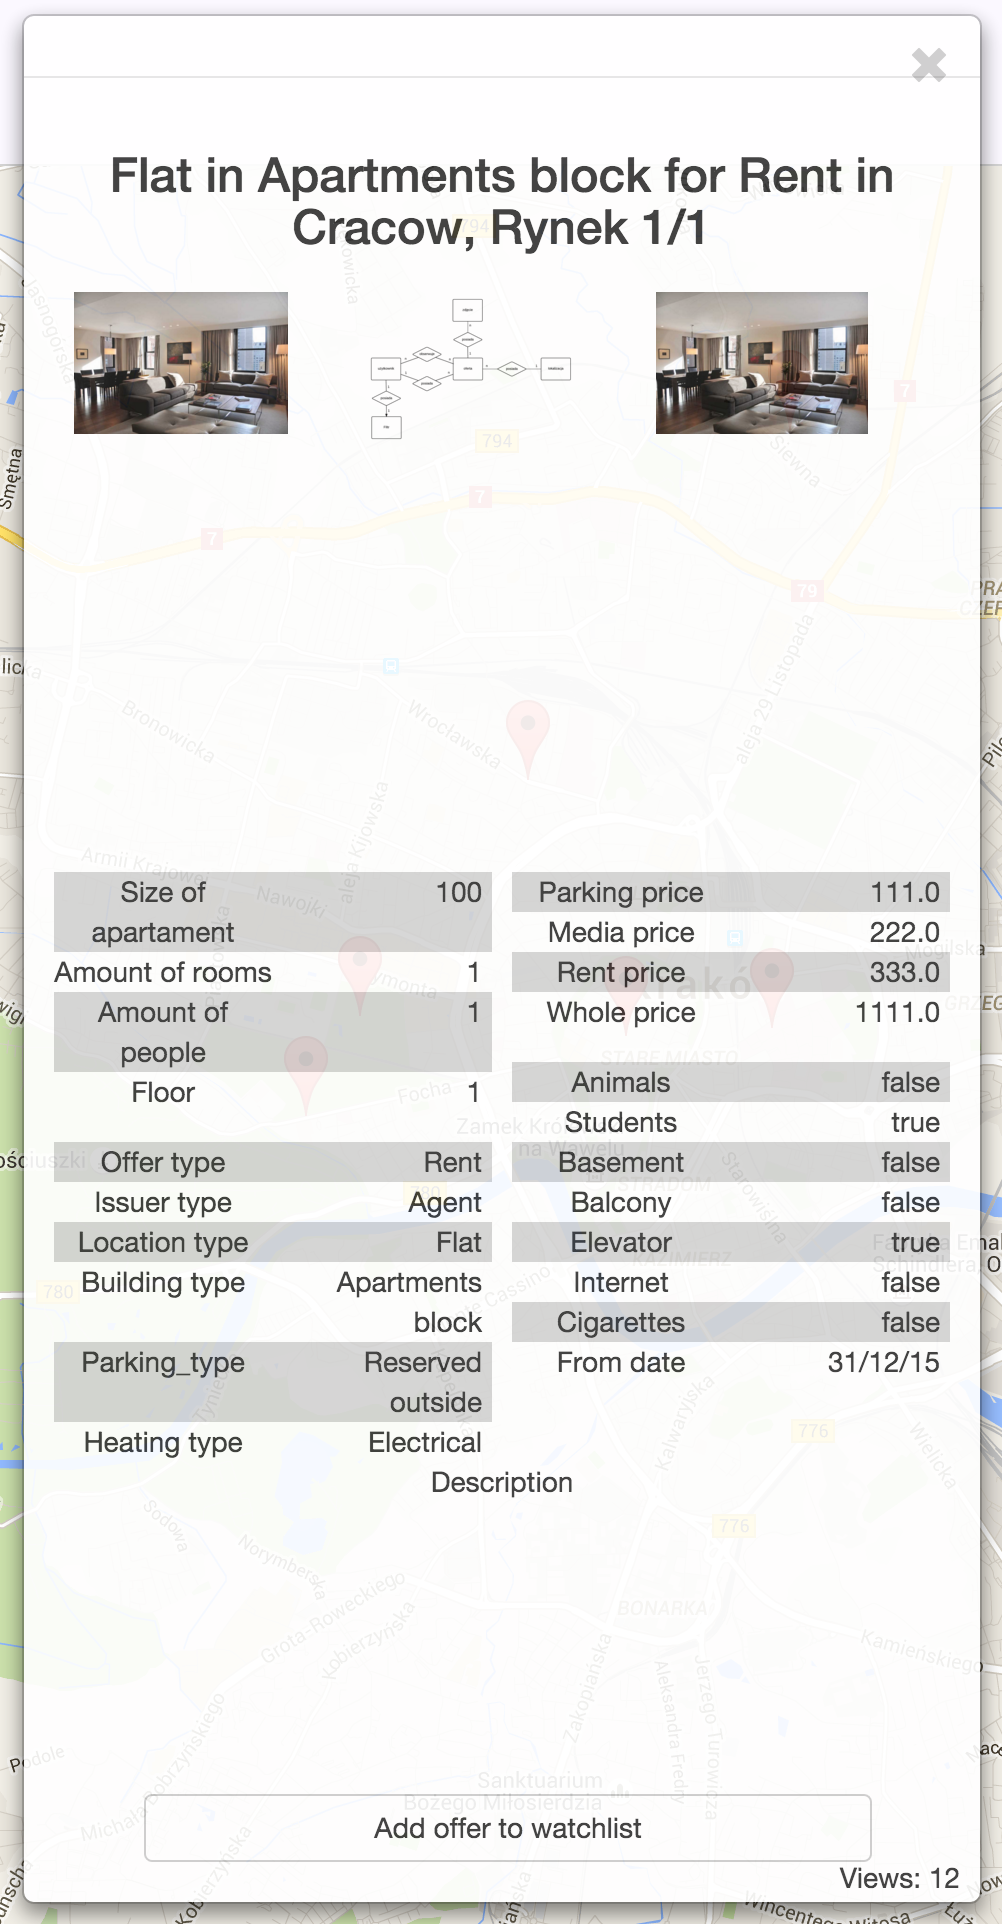
\includegraphics[keepaspectratio=true,scale=0.5]{pictures/watch-offer.png}}
\captionof{figure}{Dodawanie ofert do obserwowanych}\label{watch-offer}
\end{minipage}\\ 
